
\documentclass[a4paper,10pt]{article}
\usepackage{fullpage}
\usepackage{float}
\usepackage[english]{babel}
\usepackage{graphicx,subfig,wrapfig}
\usepackage{amsmath,amsfonts,amsthm,amssymb}
\usepackage{fancyhdr,fancybox,color}
\usepackage{enumerate}
\usepackage{multirow}
\usepackage[amssymb]{SIunits}
\definecolor{MyBlue}{rgb}{0,0.3,0.6}
\usepackage[colorlinks=true,
            linkcolor=MyBlue,
            plainpages=false,
            citecolor=MyBlue,
            urlcolor=MyBlue]{hyperref}
\usepackage[all]{hypcap}
\usepackage{tcolorbox}
\usepackage[url=false,
backend=bibtex,
style=authoryear-comp,
doi=true,
isbn=true,
backref=false,
dashed=false,
maxcitenames=2,
maxbibnames=99,
natbib=true]{biblatex}
\DeclareNameAlias{author}{last-first}
\renewbibmacro{in:}{}

\addbibresource{../_logosAndRef/references.bib}

\definecolor{mgray}{gray}{0.85}
\definecolor{mpurple}{HTML}{68236D}
\nonfrenchspacing

\begin{document}
\noindent Chair: Physics of Fluids Department
\begin{center}
 \begin{LARGE}
  Instability dynamics of flowing liquid films: on plates and fibers
 \end{LARGE}
\end{center}

\noindent Ever watched honey drip from a spoon or noticed how rainwater forms rivulets on a window? These everyday phenomena hide intriguing physics that governs industrial coating processes, heat exchangers, and microfluidic devices.


\begin{tcolorbox}[colback=mgray,colframe=mpurple,title=TL;DR]
    Liquid films flowing down inclined surfaces transition between distinct instability regimes as inclination angle varies. On plates, horizontal films remain stable while increasing angle triggers Kapitza waves, coupling with Rayleigh--Taylor instability beyond $90^\circ$. Fibers exhibit additional Rayleigh--Plateau instability forming beads. Using Basilisk CFD simulations, you'll map stability boundaries, characterize wave dynamics through spectral analysis, and identify instability coupling mechanisms. The project combines linear stability theory with direct numerical simulations to advance understanding of thin film flows relevant to coating processes and heat transfer applications.
\end{tcolorbox}

\section*{Description}

Liquid films flowing down inclined surfaces exhibit rich dynamics governed by competing instabilities. This project aims to investigate the behavior of liquid films flowing down inclined plates (figure~\ref{Figure::Typical}a) and fibers  (figure~\ref{Figure::Typical}b), focusing on the influence of the angle of inclination and the onset of various instabilities on the flow dynamics. While the behavior of films on vertical and horizontal surfaces are well-studied, the transition between different instability regimes as inclination angle $\theta$ varies from $0^\circ$ to $180^\circ$ remains open to further investigation.

\section*{Deep dive}
The two systems under study are a liquid film flowing down an inclined plane and a liquid film streaming down an inclined fiber. Both systems are driven by gravity and are subject to instabilities that can significantly influence their flow dynamics. However, they exhibit different behaviors and are subject to different types of instabilities due to their distinct geometries.

In the case of a liquid film flowing down an inclined plane \citep{craster2009dynamics}, the stability of the film is determined by the angle of the plane. When the plane is horizontal, the film is stable. As the angle increases, Kapitza instability occurs, characterized by the formation of waves on the surface of the liquid film. As the angle increases, particularly beyond 90 degrees, Kapitza instability couples with Rayleigh-Taylor instability as the liquid drips. When the plane reaches 180 degrees, only Rayleigh-Taylor instability remains.

On the other hand, a liquid film flowing down a vertical fiber is an unstable open-flow hydrodynamic system that exhibits a variety of wave phenomena and transitions \citep{kalliadasis1994drop, quere1999fluid, kliakhandler2001viscous, craster2006viscous}. This is due to the interplay between Kapitza instability, common in films falling down vertical planes, and Rayleigh--Plateau instability, typical in a liquid layer coating a cylinder. These instabilities can lead to the formation of bead-like patterns on the fiber, which are desirable in applications where heat and mass transfer across a liquid-gas interface occurs.

Through this research, we aim to provide a comprehensive understanding of the behavior of liquid film flows on inclined fibers \citep{pour2023experimental} and plates \citep{craster2009dynamics}, contributing to the broader field of fluid dynamics.

\begin{figure}
	\begin{center}
		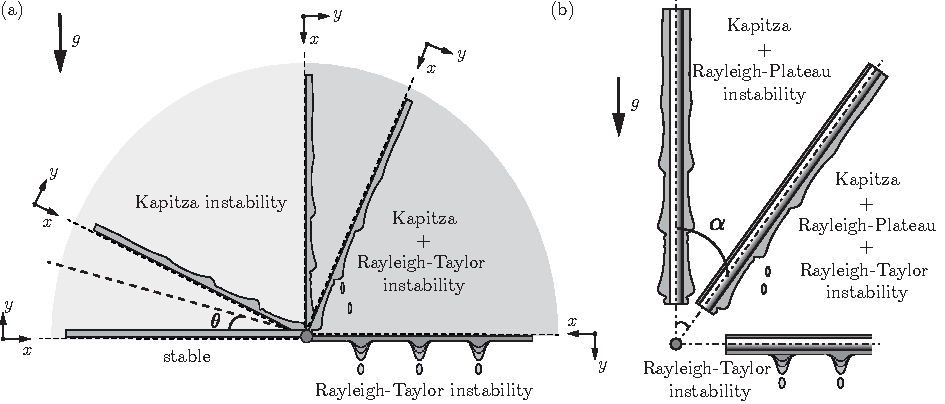
\includegraphics[width=0.8\textwidth]{schematic_dropsOnFibers.pdf}
		\caption{Schematic of the problem: (a) Liquid film flowing down an inclined plate. As the angle of inclination ($\theta$) changes, different instabilities kick in, starting from the convective Kapitza instability, which couples with Rayleigh-Taylor instability after a critical angle of inclination is reached. (b) Liquid film flowing down a fiber. For a vertical fiber, Kapitza and Rayleigh-Plateau instability dominate. However,  as a critical inclination is reached, Rayleigh-Taylor instability dominates, particularly as the inclination angle approaches $\pi$. Figure adapted from \citet{rietz2017dynamics}.}
		\label{Figure::Typical}
\end{center}
\end{figure}

\noindent The main objectives of this study are:

\begin{enumerate}
	\item How does the angle of inclination influence the stability of liquid films on fibers and plates? We will systematically vary the angle of inclination and observe the resulting changes in the stability and flow dynamics of the liquid films.
	
	\item How does the transition between different instabilities occur as the angle of inclination changes? We will conduct detailed numerical simulation to capture the transition points between different instabilities and understand the underlying mechanisms (see figure~\ref{Figure::Typical}). 
	
	\item How do different instabilities interact and influence the flow dynamics of liquid films? We will study the interactions between Kapitza, Rayleigh-Taylor, and Rayleigh-Plateau instabilities and their collective impact on the flow dynamics.
	
	\item What are the underlying mechanisms that govern the gravity-driven flow of liquid film down an incline or a fiber?
		
	\item To identify and explore the different timescales relevant for this process (see the introduction of \citet{VatsalThesis}).
\end{enumerate}

\section*{What will you do and what will you learn?}
For this project, we are looking for enthusiastic students to work on this topic.
\begin{enumerate}
\itemsep0em
\item You will learn about fundamental fluid dynamics.
\item You will get hands-on experience with Computational Fluid Dynamics (CFD).
\item You will learn how to do basic and advanced data analysis.
%\item You will learn modeling of complex multiphase systems contact lines. 
\item You will learn how to document and publish read-to-use codes and share them with the community, similar to \citet{basiliskVatsal, basiliskVatsalDropFilm, basiliskVatsalViscousBouncing}. 
\item As a part of the \href{https://comphy-lab.org}{CoMPhy lab}, you will learn and adapt open-source coding principles. 

\end{enumerate}

If you have any questions, fell free to contact \href{mailto:vatsal.sanjay@comphy-lab.org}{Vatsal} (details below).
\begin{center}
\begin{tabular}{|l|l|l|}
\hline \textbf{Supervision} & \textbf{E-mail} & \textbf{Office} \\
\hline \multirow{2}{*}{Dr. Vatsal Sanjay} & \href{mailto:vatsal.sanjay@comphy-lab.org}{vatsal.sanjay@comphy-lab.org} & \multirow{2}{*}{Durham University} \\
& \href{mailto:vatsal.sanjay@durham.ac.uk}{vatsal.sanjay@durham.ac.uk} & \\
\hline Jnandeep Talukdar M.Sc. & \href{mailto:jnandeep.iitp@gmail.com}{jnandeep.iitp@gmail.com} & Meander 246B \\
\hline Prof. Dr.-Ing. Wilko Rohlfs   & \href{mailto:w.rohlfs@utwente.nl}{w.rohlfs@utwente.nl}& Horst Complex, N234 \\
\hline Prof. Dr. Detlef Lohse F.R.S. & \href{mailto:d.lohse@utwente.nl}{d.lohse@utwente.nl} & Meander 261  \\
\hline
\end{tabular}
\end{center}

\printbibliography

\end{document}
